\documentclass[border=3pt]{standalone}
% Preâmbulo compartilhado pelos diagramas TikZ da aula 7 de IHR (Emoção)
\usepackage[T1]{fontenc}
\usepackage[utf8]{inputenc}
\usepackage{lmodern}
\usepackage{amsmath}
\usepackage{xcolor}
\usepackage{tikz}
\usetikzlibrary{arrows.meta,angles,quotes,decorations.pathmorphing,decorations.pathreplacing,calc,
                positioning,shapes.geometric,shapes.misc,backgrounds,fit,
                math}

% Paleta (mesma dos SVGs originais)
% Paleta da disciplina de IHR: acento azul (#1A6FB5), cor de destaque do tema.
% (o nome "dblue" é mantido para não alterar todos os diagramas)
\definecolor{dblue}{HTML}{1A6FB5}
\definecolor{dorange}{HTML}{B3541E}
\definecolor{dgreen}{HTML}{4A7C59}
\definecolor{dred}{HTML}{9C4B4B}
\definecolor{dcream}{HTML}{F4F1EA}
\definecolor{dshade}{HTML}{DDD7C9}

% Função gaussiana (não normalizada por padrão de escala visual)
\pgfmathdeclarefunction{gauss}{3}{%
  \pgfmathparse{1/(#3*sqrt(2*pi))*exp(-((#1-#2)^2)/(2*#3^2))}%
}

% Estilos comuns (prefixo d... para não colidir com chaves internas do pgf)
\tikzset{
  >={Stealth[length=2mm]},
  dguide/.style={gray!55, dashed, line width=0.4pt},
  daxis/.style={gray!60, line width=0.7pt, ->},
  dbody/.style={fill=black!3, draw=black!80, line width=1pt},
  dacc/.style={draw=dblue, line width=1pt},
  dlbl/.style={black!55, font=\small},
  dsub/.style={black!45, font=\footnotesize},
  dstate/.style={circle, draw=black!80, fill=dcream, line width=1pt,
                 minimum size=17mm, font=\large, inner sep=1pt},
  dobs/.style={circle, draw=black!80, fill=dshade, line width=1pt,
               minimum size=14mm, font=\large, inner sep=1pt},
  dbox/.style={rounded corners=2pt, draw=black!80, fill=dcream, line width=1pt,
               align=center, inner sep=6pt},
  dop/.style={circle, draw=black!80, fill=white, line width=1pt,
              minimum size=6mm, inner sep=0pt, font=\small},
  dtrans/.style={->, dblue, line width=1pt},
  dmeas/.style={->, dorange, line width=1pt},
  dcurve/.style={line width=1pt, dblue},
  dcurveb/.style={line width=1.4pt, dorange},
}

\begin{document}
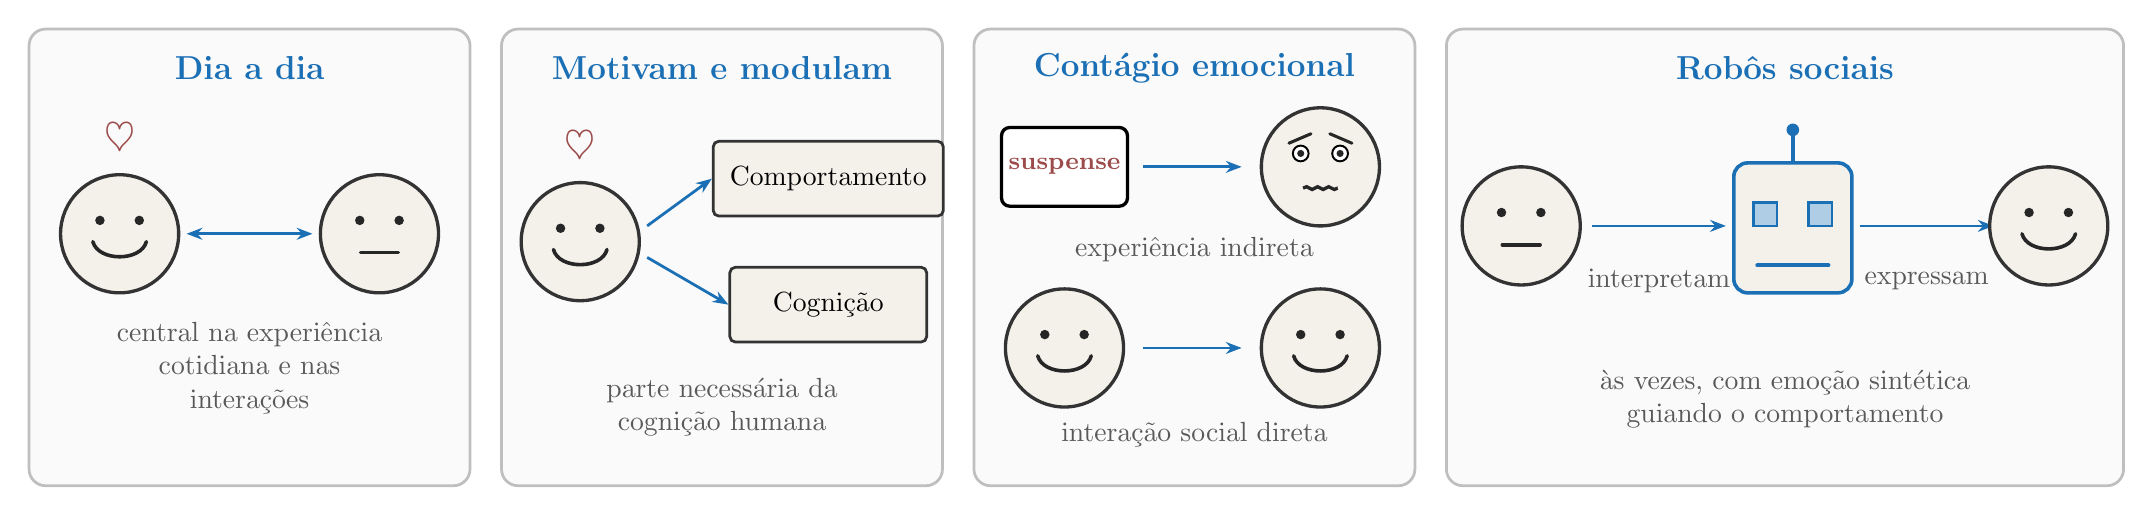
\begin{tikzpicture}[x=1cm,y=1cm]

  \tikzset{
    hd/.style={circle, draw=black!80, fill=dcream, line width=1.2pt, minimum size=1.5cm},
    cell/.style={draw=black!25, rounded corners=6pt, line width=1pt, fill=black!2},
    ttl/.style={font=\large\bfseries, dblue},
    lab/.style={font=\normalsize, black!65, align=center},
    box/.style={dbox, font=\large, minimum height=0.95cm, minimum width=2.6cm},
    arr/.style={line width=1.4pt, -{Stealth[length=2.6mm]}, dtrans}}
  % rostos: centro (x,y)
  \newcommand{\happy}[2]{\node[hd] at (#1,#2) {};
    \fill[black!85] (#1-0.25,#2+0.17) circle (0.06) (#1+0.25,#2+0.17) circle (0.06);
    \draw[black!85, line width=1.3pt, line cap=round] (#1-0.34,#2-0.1) to[bend right=75] (#1+0.34,#2-0.1);}
  \newcommand{\neutral}[2]{\node[hd] at (#1,#2) {};
    \fill[black!85] (#1-0.25,#2+0.17) circle (0.06) (#1+0.25,#2+0.17) circle (0.06);
    \draw[black!85, line width=1.3pt, line cap=round] (#1-0.24,#2-0.24) -- (#1+0.24,#2-0.24);}
  \newcommand{\tense}[2]{\node[hd] at (#1,#2) {};
    \draw[fill=white, line width=0.7pt] (#1-0.25,#2+0.17) circle (0.1) (#1+0.25,#2+0.17) circle (0.1);
    \fill[black!85] (#1-0.25,#2+0.17) circle (0.045) (#1+0.25,#2+0.17) circle (0.045);
    \draw[black!85, line width=1.1pt, line cap=round] (#1-0.4,#2+0.3) -- (#1-0.12,#2+0.42) (#1+0.4,#2+0.3) -- (#1+0.12,#2+0.42);
    \draw[black!85, line width=1.2pt, decorate, decoration={snake, amplitude=0.5pt, segment length=4pt}] (#1-0.22,#2-0.27) -- (#1+0.22,#2-0.27);}

  % ============ A: dia a dia e interações ============
  \begin{scope}[shift={(0,0)}]
    \draw[cell] (0,0) rectangle (5.6,5.8);
    \node[ttl] at (2.8,5.3) {Dia a dia};
    \happy{1.15}{3.2}
    \neutral{4.45}{3.2}
    \draw[arr, <->] (2.0,3.2) -- (3.6,3.2);
    \node[dred, font=\Large] at (1.15,4.4) {\ensuremath{\heartsuit}};
    \node[lab] at (2.8,1.5) {central na experiência\\ cotidiana e nas\\ interações};
  \end{scope}

  % ============ B: motivam e modulam ============
  \begin{scope}[shift={(6.0,0)}]
    \draw[cell] (0,0) rectangle (5.6,5.8);
    \node[ttl] at (2.8,5.3) {Motivam e modulam};
    \happy{1.0}{3.1}
    \node[dred, font=\Large] at (1.0,4.3) {\ensuremath{\heartsuit}};
    \node[box, font=\normalsize, minimum width=2.5cm] (b1) at (4.15,3.9) {Comportamento};
    \node[box, font=\normalsize, minimum width=2.5cm] (b2) at (4.15,2.3) {Cognição};
    \draw[arr] (1.85,3.3) -- (b1.west);
    \draw[arr] (1.85,2.9) -- (b2.west);
    \node[lab] at (2.8,1.0) {parte necessária da\\ cognição humana};
  \end{scope}

  % ============ C: contágio ============
  \begin{scope}[shift={(12.0,0)}]
    \draw[cell] (0,0) rectangle (5.6,5.8);
    \node[ttl] at (2.8,5.3) {Contágio emocional};
    \draw[line width=1.2pt, fill=white, rounded corners=3pt] (0.35,3.55) rectangle (1.95,4.55);
    \node[font=\small\bfseries, dred] at (1.15,4.05) {suspense};
    \draw[arr] (2.15,4.05) -- (3.4,4.05);
    \tense{4.4}{4.05}
    \node[lab] at (2.8,3.0) {experiência indireta};
    \happy{1.15}{1.75}
    \draw[arr] (2.15,1.75) -- (3.4,1.75);
    \happy{4.4}{1.75}
    \node[lab] at (2.8,0.65) {interação social direta};
  \end{scope}

  % ============ D: robôs sociais ============
  \begin{scope}[shift={(18.0,0)}]
    \draw[cell] (0,0) rectangle (8.6,5.8);
    \node[ttl] at (4.3,5.3) {Robôs sociais};
    \neutral{0.95}{3.3}
    \draw[arr] (1.85,3.3) -- (3.55,3.3);
    \node[lab] at (2.7,2.6) {interpretam};
    \draw[line width=1.3pt, draw=dblue, fill=dcream, rounded corners=5pt] (3.65,2.45) rectangle (5.15,4.1);
    \draw[draw=dblue, line width=1.3pt] (4.4,4.1) -- (4.4,4.45); \fill[dblue] (4.4,4.52) circle (0.08);
    \fill[dblue!35, draw=dblue, line width=0.9pt] (3.9,3.3) rectangle (4.2,3.6) (4.6,3.3) rectangle (4.9,3.6);
    \draw[dblue, line width=1.5pt, line cap=round] (3.95,2.8) -- (4.85,2.8);
    \draw[arr] (5.25,3.3) -- (6.95,3.3);
    \node[lab] at (6.1,2.6) {expressam};
    \happy{7.65}{3.3}
    \node[lab] at (4.3,1.1) {às vezes, com emoção sintética\\ guiando o comportamento};
  \end{scope}

\end{tikzpicture}
\end{document}
